\section{Zufallsvariablen}
Bei einem Zufallsexperiment \wraum\ interessiert man sich oft nicht für das
Ergebnis $\w \in \tO$ sondern für eine Kennzahl $X(\w)$, die von \w\ abhängt.

\paragraph{Beispiel:} n-maliges Würfeln.\\
$\tO  = \{1,2,3,4,5,6\}^n = \{ \w = (\w_1, \dots, \w_n): \w_i \in \{1, \dots, 6\} \; \forall i=1, \dots, n$ \}\\
Mögliche Kennzahlen $X(\w)$ wären:
\begin{align*}
    X(\w) & = \min \w_k \\
    X(\w) & = \max \w_k \\
    X(\w) & = \sum \w_k
\end{align*}

\begin{definition}[Zufallsvariable]
    \label{def:zufallsvar}
    Sei \wraum\ ein W-Raum und $X: \tO \to \real$ eine Abbildung.
    $X$ heißt Zufallsvariable, falls für alle $B \in B(\real)$ gilt:
    \begin{equation*}
        \underbrace{\{\w \in \tO: X(\w) \in B\}}_{\subset \tO} \in \tS
    \end{equation*}
\end{definition}

\paragraph{Bemerkungen}
\begin{enumerate}
    \item Zufallsvariablen sind Abbildungen
    \item Die Aussage aus \autoref{def:zufallsvar} muss hier nicht überprüft
          werden.
          Alle im folgenden auftauchenden Abbildungen sind Zufallsvariablen.
    \item Wir schreiben $\{X \in B\}$ für das Ereignis
          $\{\w \in \tO: X(\w) \in B\}$.
\end{enumerate}

\begin{definition}[Verteilung einer Zufallsvariable]
    Sei $X: \tO \to \real$ eine Zufallsvariable und \wraum\ ein W-Raum.
    Dann heißt das W-Maß $P_X: B(\real) \to [0,1]$ mit
    $P_X(B) = P(\{X \in B\}) = P(\{\w \in \tO: X(\w) \in B\})$, $B \in B(\real)$,
    die \emph{Verteilung} von $X$.
\end{definition}

\todo{Übung: Angeben von Verteilung mit Bsp}

\paragraph{Beachte:}
$X$ bildet den ursprünglichen W-Raum in einen neuen ab:
\begin{center}
    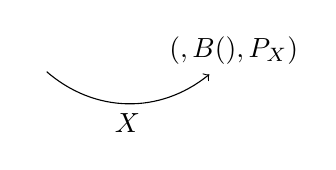
\begin{tikzpicture}
        \node[anchor=south] (a) at (0,0) {\wraum};
        \node[anchor=south] (b) at (2.5,0) {$(\real, B(\real), P_X)$};
        \path[->] (a) edge[bend right=40] node[below]{$X$} (b);
    \end{tikzpicture}
\end{center}

\subsection{Diskrete Verteilungen}

\begin{definition}[Diskrete Zufallsvariablen]
    \begin{enumerate}
        \item Eine Zufallsvariable heißt diskret, falls eine Menge $D \subset \real$
              existiert, die höchstens abzählbar ist mit $P(\{X \in D\})=1$.
        \item Sei $X$ diskret. Die Menge $D_X = \{ x \in \real: P(\{X \in D\})>0 \}$
              heißt der \emph{Träger} von $X$.\\
              Beachte: Es gilt $P(\{X \in D_X \}) = 1$.
    \end{enumerate}
\end{definition}

\begin{enumerate}
    \item $X$ heißt \emph{Bernoulli} verteilt mit Parameter $p \in [0,1]$, falls gilt:
          \begin{align*}
              P(\{X=1\}) & = p   \\
              P(\{X=0\}) & = 1-p
          \end{align*}
          In diesem Fall gilt: $P(\{X\in\underbrace{\{0,1\}}_{=D}\}) = p+(1-p) = 1$
          Ferner gilt:
          \begin{equation*}
              D_X = \begin{cases}
                  \{0,1\} & , \text{falls } p \in (0,1) \\
                  \{0\}   & , \text{falls } p=0         \\
                  \{1\}   & , \text{falls } p=1
              \end{cases}
          \end{equation*}
          Wir schreiben:
          \begin{equation*}
              X \sim B(1,p)
          \end{equation*}

    \item $X$ heißt \emph{Gleichverteilt} auf $G$, für $G \subset \real$, $G \neq \emptyset$
          und endlich, falls
          \begin{equation*}
              P(\{X=x\}) = \frac{1}{|G|} \; \forall x \in G
          \end{equation*}
          Wir schreiben:
          \begin{equation*}
              X \sim U(G)
          \end{equation*}

    \item $X$ heißt \emph{hypergeometrisch} verteilt mit Parametern
          \begin{align*}
              n & \in \mathbb{N}      & \textit{Anzahl Kugeln}   \\
              B & \in \{0, \dots, n\} & \textit{blaue Kugeln}    \\
              k & \in \{1, \dots, n\} & \textit{gezogene Kugeln} \\
          \end{align*}
          wenn gilt:
          \begin{equation*}
              P\left(\left\{X=b\right\}\right)
              = \frac{\binom{B}{b} \binom{n-B}{k-b}}{\binom{n}{k}}
          \end{equation*}
          Wir schreiben:
          \begin{equation*}
              X \sim H(n,B,k)
          \end{equation*}

    \item $X$ heißt \emph{Poissonverteilt} mit Parameter $\lambda > 0$, falls gilt:
          \begin{equation*}
              P(\{X=k\}) = \frac{\lambda^k}{k!} e^{-\lambda} \;\; \forall k\in \mathbb{N}_0
          \end{equation*}
          Wir schreiben:
          \begin{equation*}
              X \sim P(\lambda)
          \end{equation*}

    \item $X$ heißt \emph{geometrisch} verteilt mit Parameter $p \in (0,1]$, falls
          \begin{equation*}
              P(\{X=k\}) = p (1-p)^{k-1} \;\; \forall k \in \mathbb{N}
          \end{equation*}
          Wir schreiben:
          \begin{equation*}
              X \sim G(p)
          \end{equation*}
\end{enumerate}

\subsection{Verteilungsfunktion}

\begin{definition}[Verteilungsfunktion]
    Ist $X$ eine Zufallsvariable auf \wraum, dann ist die Verteilungsfunktion
    $F_X: \real \to [0,1]$ von $X$ gegeben durch
    \begin{equation*}
        F_X(t) = P(\{X \leq t\})
    \end{equation*}
\end{definition}

\subsubsection{Verteilungsfunktion einer diskreten Zufallsvariable}
\begin{equation*}
    F_X(t) = \sum_{k=0}^t P(\{X=k\})
\end{equation*}
$P(\{X=k\})$ ist die \emph{Zähldichte} von $X$.
\todo{Zähldichte: Tut 3}

\subsubsection{Verteilungsfunktion einer absolut stetigen Zufallsvariable}
\begin{equation*}
    F_X(t) = \int_{-\infty}^t p(x) dx
\end{equation*}
$p(x)$ ist die \emph{Wahrscheinlichkeitsdichte} von $X$.

\subsubsection{Eigenschaften der Verteilungsfunktion}
\begin{itemize}
    \item $F_X$ ist monoton wachsend
    \item Grenzwerte:
          \begin{align*}
              \lim_{t \to -\infty} F_X(t) = 0 \\
              \lim_{t \to \infty} F_X(t) = 1  \\
          \end{align*}
    \item $F_X$ ist rechtsseitig stetig:
          \begin{equation*}
              \lim_{t_n \uparrow t} F_X(t_n) = F_X(t)
          \end{equation*}
    \item Für jedes $t \in \real$ existiert der linksseitige Grenzwert:
          \begin{equation*}
              F_X(t-) = \lim_{t_n \downarrow t} F_X(t_n)
          \end{equation*}
    \item Es gilt:
          \begin{equation*}
              P(\{X=t\}) = F_X(t) - F_X(-t)
          \end{equation*}
    \item Für $a<b$ gilt:
          \begin{equation*}
              P(\{X \in [a,b]\}) = \int_a^b p(x)dx
          \end{equation*}
    \item Die Verteilung einer Zufallsvariable ist eindeutig durch ihre Verteilungsfunktion
          bestimmt.
\end{itemize}

\subsection{Beispiele}
\subsubsection{Definition einer Zufallsvariable}
In Übungsblatt 6 wurde die Aufgabe gestellt:
\say{Modellieren Sie das Zufallsexperiment durch Angabe eines geeigneten Wahrscheinlichkeitsraumes und definieren Sie $X$}

Der W-Raum kann unabhängig von der Zufallsvariablen durch Betrachten des Experiments
aufgestellt werden.
Das Beispiel hier ist das 3-malige Drehen eines Glücksrads, mit gleichen Wahrscheinlichkeiten.
Es wird ein Laplace Raum mit $\tO = \{1,2,3\}^3$ angegeben. \tS\ als Potenzmenge und
$P(A) = \frac{|A|}{|\tO|}$ folgt aus der Tatsache dass es sich um einen Laplace Raum handelt.

Für $X: \tO \to \real$ genügt es, eine Vorschrift $X(\w)$, hier
$X(\w) = \w_1 \cdot \w_2 \cdot \w_3$ mit $\w = (\w_1, \w_2, \w_3)$, anzugeben.
